\chapter{基于预测的容器弹性服务策略 }\label{chap:elastic_service}

\section{引言}

在本文前面的章节中,设计了基于容器化的多终端协同服务系统,将位于用户终端边缘的多个智能终端设备上的空余资源整合起来,以容器的形式为用户终端提供服务,以提高终端资源的利用率,提高终端用户的体验。但是在智能终端上以容器的形式对外提供服务的时候,会出现一组矛盾的问题。如果采用预部署的形式,即在边缘终端上提前部署好提供服务的容器,那么收到用户的服务请求就可以马上对外提供服务。但由于智能终端的资源是有限的,终端服务不能像云端系统服务那样一直在后台运行,等待着用户请求流量的到达。这种预部署的方式使得提供服务的容器也会·消耗智能终端上面的资源,在用户请求流量较低的时候会造成一种智能终端资源的浪费。如果采用非预部署的形式,即不提前部署容器,而是等到用户请求到达服务终端以后再临时创建容器提供服务,在服务完成后可以看情况销毁容器,这样就可以减小很多额外开销,节约智能终端的资源。但是这种非预部署的形式会大大增加用户的平均等待时间,因为相比一次服务的计算和网络传输开销,一次容器创建的时间还是非常长的,对于等待服务请求响应的用户来说完全不能够接受。

为了解决多终端协同服务技术中的预部署问题,促进提高终端资源利用率和降低用户服务请求响应等待时间之间的平衡,我们提出基于预测的容器弹性服务策略,根据预测结果提前弹性部署容器服务,动态调整多终端协同服务的规模,平衡提高终端资源利用率与降低用户服务请求响应等待时间之间的关系。本章提出的基于预测的容器弹性服务策略,具体实现为第\ref{chap:service_system}章中所提出的系统架构设计中的弹性服务模块。

本章的内容组织结构如下:第\ref{sec:elastic_service_related_work}节介绍了预测算法的相关研究工作,包括基于统计学模型的预测算法和基于卡尔曼滤波的预测算法;第\ref{sec:elastic_service_Kalman_filtering}节介绍了多终端协同服务中的用户流量预测模型,以及卡尔曼滤波预测算法,并结合多终端协同服务技术场景的特点,提出一种改进的卡尔曼滤波预测算法;第\ref{sec:elastic_service_strategy}节介绍了基于预测的容器弹性服务策略的设计思路,对具体弹性服务策略的流程进行了设计;第\ref{sec:elastic_service_experiment_results}节列出了仿真实验的结果及分析;第\ref{sec:elastic_service_summary}节总结了本章内容。

\section{相关工作}\label{sec:elastic_service_related_work}

\subsection{基于统计学模型的预测算法}

早期的网络流量预测算法是简单地基于统计学模型来进行预测的,典型的如基于泊松模型、马尔可夫过程及增量高斯混合模型。但是这些简单的模型并不能很好地满足网络流量多变的状况。
灰度模型

\subsection{基于卡尔曼滤波器的预测算法}

1960年,数学家卡尔曼提出了卡尔曼滤波器(Kalman Filtering)\cite{kalman1960new}。卡尔曼滤波器是一种最优化自回归数据处理算法,这种方法通过对预测值与真实测量值进行方差加权来获得新的预测值,通过迭代不断进行预估与校正\cite{彭丁聪2009卡尔曼滤波的基本原理及应用}。对于一个确定性未知的动态系统来说,卡尔曼滤波器可以在考虑噪声信息干扰的情况下,对于系统的过去、现在以及未来的状态做出较为准确的估计\cite{muruganantham2016evolutionary}。由于效率非常高,卡尔曼滤波器被应用于包括运动轨迹预测\cite{成光2006基于卡尔曼滤波的目标估计和预测方法研究}、电网负荷预测\cite{刘鑫2019基于改进卡尔曼滤波算法的短期负荷预测}、气象数据融合\cite{周艳青2018基于改进的卡尔曼滤波算法的气象数据融合}等多个领域。文献\cite{郝庭毅2017面向微服务架构的容器级弹性资源供给方法}中针对微服务架构,提出了一种利用模糊自适应卡尔曼滤波算法来对服务响应时间进行预测。文献\cite{贾濡2018基于卡尔曼滤波的流量预测机制}针对智慧协同网络(SINET),利用卡尔曼滤波算法对网络流量进行预测。

卡尔曼滤波器的预测模型非常简单,只需要保存当前状态的一些统计信息,即可对系统的下一个状态进行预测,具有容易实现的优点。而且卡尔曼滤波器计算简单,运行速度快,占用计算资源和存储资源少,相比前面提到的算法,与本文提出的基于容器化的多终端协同服务技术的应用场景更加适合。

\section{基于卡尔曼滤波的预测算法}\label{sec:elastic_service_Kalman_filtering}
\subsection{卡尔曼滤波器}

卡尔曼滤波器的表达式是一组数学方程,能够提供最小二乘法的有效递归解\cite{welch1995introduction}。为了利用卡尔曼滤波器来解决本章中所提出的容器弹性服务问题,需要将该问题用数学表达式来描述。在本研究所提出的基于容器化的多终端协同服务技术中,通过对用户的服务请求流量的趋势进行预测,动态调整容器服务集群规模,以达到提供容器弹性服务的目的。该系统可以用表达式\ref{equ:describe_x_k}来描述,系统中所有变量均为一维变量。

\begin{equation}\label{equ:describe_x_k}
    X_k=AX_{k-1}+BU_{k}+W_{k}
\end{equation}

在公式\ref{equ:describe_x_k}中,$X_k$为系统在k时刻接收到的用户服务请求数量,$U_{k}$为\emph{k}时刻系统的控制变量,$W_k$为系统过程噪声,假设为高斯白噪声(White Gaussian Noise),协方差为Q。\emph{A}和\emph{B}为系统参数。

而对于系统的测量模型,表达式如公式\ref{equ:task_scheduling_makespan}所示。

\begin{equation}\label{equ:measure_x_k}
    Z_k=HX_{k}+V_{k}
\end{equation}

在公式\ref{equ:measure_x_k}中,$Z_k$是系统\emph{k}时刻的测量值,$V_k$为系统的测量噪声,同样假设为高斯白噪声,协方差为R。\emph{H}为测量系统的参数。

卡尔曼滤波器可以分为预估和校正两个阶段\cite{彭丁聪2009卡尔曼滤波的基本原理及应用}。在预估阶段中,系统根据时间更新方程及上一时刻系统的状态,对当前时刻的状态进行先验预估,并计算先验估计的协方差。而在校正阶段,系统通过测量的方法获得系统当前状态的观测值,通过状态更新方程计算出卡尔曼滤波增益,并对预估阶段中得到的先验估计值进行校正,得到系统当前时刻状态的后验估计值。当前时刻状态的后验估计值在下一时刻又可以根据时间更新方程计算下一时刻的系统状态先验估计。如此循环迭代,即可对系统的状态进行预测和跟踪。

离散卡尔曼滤波的时间更新方程如公式\ref{equ:kalman_time_1}和公式\ref{equ:kalman_time_2}所示。
\begin{equation}\label{equ:kalman_time_1}
    X_k=AX_{k-1}+BU_k
\end{equation}

\begin{equation}\label{equ:kalman_time_2}
    P_k=A^2P_{k-1}+Q
\end{equation}

在公式\ref{equ:kalman_time_2}中的$P_k$为先验估计的方差。离散卡尔曼滤波的状态更新方程如公式\ref{equ:kalman_status_1}、公式\ref{equ:kalman_status_2}和公式\ref{equ:kalman_status_3}所示。

\begin{equation}\label{equ:kalman_status_1}
    K_k=HP_k(H^2P_k+R)^{-1}
\end{equation}

\begin{equation}\label{equ:kalman_status_2}
    \widehat{X_k}=X_k+K_{k}(Z_k-HX_k)
\end{equation}

\begin{equation}\label{equ:kalman_status_3}
    \widehat{P_k}=(1-K_kH)P_k
\end{equation}

在公式\ref{equ:kalman_status_2}中的$\widehat{X_k}$为对\emph{k}时刻系统状态的后验估计。在公式\ref{equ:kalman_status_3}中的$\widehat{P_k}$为对\emph{k}时刻系统误差的后验估计。

\subsection{基于终端服务的改进卡尔曼滤波算法}

我们利用卡尔曼滤波器的方法,采集历史用户请求数据,并对下一时间点的用户请求数量进行预测,弹性调整容器服务规模。基于卡尔曼滤波的预测方法计算量相对比较小,适合在基于容器化的多智能终端协同服务技术的场景中应用。但是由于我们的应用场景对于网络波动比较敏感,对预测的精度可以适当放宽要求,因此可以考虑基于终端服务的特点,对基于卡尔曼滤波的预测方法进行一定优化,以期能够提早发现网络流量的突然变化。而适当放弃预测的准确度,即出现一定程度的误报是可以接受的。
选择已有的网络排队模型,利用卡尔曼滤波的方法获取预测值与实际测量值,计算方差,选择权重进行迭代更新,实现对于网络流量的预测。


% 需要提出一个简单的修改,加个公式和流程图

\section{基于预测的容器弹性服务策略设计}\label{sec:elastic_service_strategy}

基于改进卡尔曼滤波预测方法的容器弹性服务的部署策略为,在开始的时候部署少部分容器用于提供初始的服务并获取初始的流量数据,当预测流量快要超过阈值的时候,适当扩大容器数量,当预测流量减小到一定程度,适当关闭一些容器并回收响应资源。这里需要注意的问题是如何选择合适的阈值,以及扩容缩容程度是怎么样的,需要结合一些理论进行研究。同时,可以对服务的平均时间进行监控,建立反馈机制,动态调节参数。模块流程图如图\ref{fig:elastic_service_system}所示。

\begin{figure}[htbp]
    \centering
    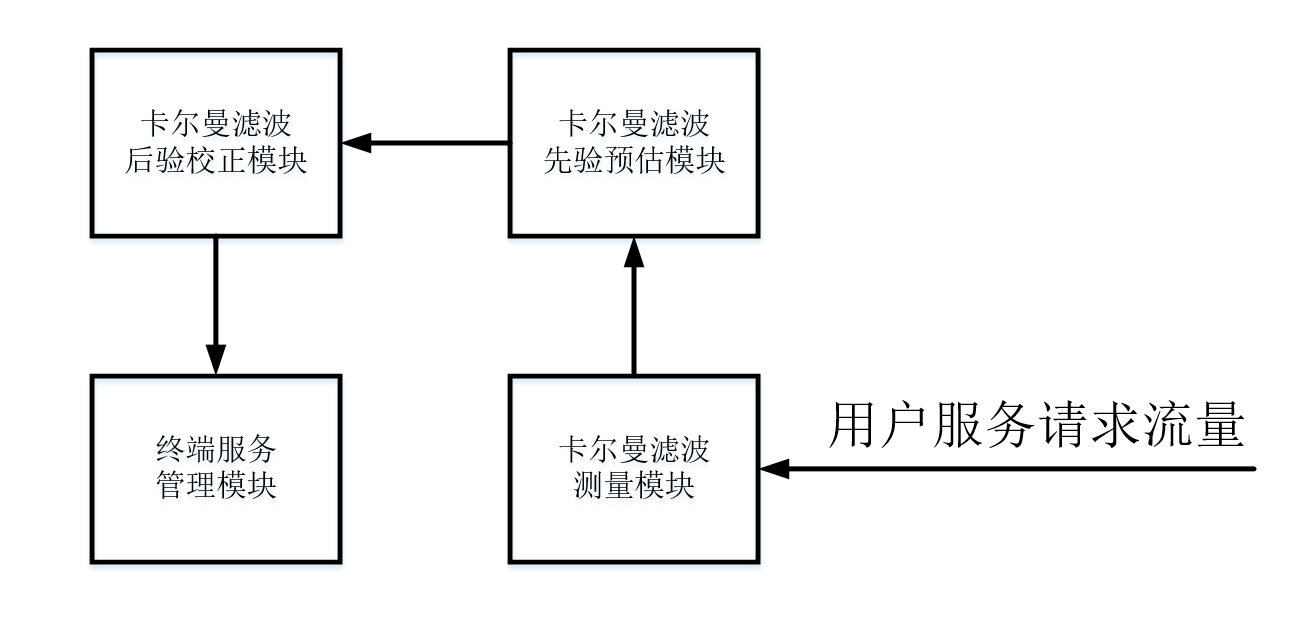
\includegraphics[width=1\linewidth]{Elastic_Service_System_temp}\hfill\\[0.5cm]
  \caption{基于预测的容器弹性服务模块图}
  \label{fig:elastic_service_system}
  \end{figure}

% 在这个模型里,还需要考虑一下,流量变化到什么程度才能进行扩容缩容,而不是一有变化就调整

% 加个流程图

\section{实验结果}\label{sec:elastic_service_experiment_results}

\section{本章小结}\label{sec:elastic_service_summary}

为了解决多终端协同服务技术中的预部署问题,促进提高终端资源利用率和降低用户服务请求响应等待时间之间的平衡,本章提出了基于预测的容器弹性服务策略。基于卡尔曼滤波器,结合多终端协同服务的特点,提出了一种改进卡尔曼滤波算法。根据预测结果提前弹性部署容器服务,动态调整多终端协同服务的规模,平衡提高终端资源利用率与降低用户服务请求响应等待时间之间的关系。